
% --- GENERIC SIMULATIONS ------------------------------------------------

\subsection{Benchmarking branch GRM and PCA computations}

% Paragraph on introducting benchmarks
We assessed the computational efficiency of different implementations of
branch GRM and PCA computation via simulation.
%
In brief, we measured the time taken to compute the branch GRM or PCA
with varying number of sample nodes and total genome sequence length.
%

All computations were carried out on a single CPU with 4GB of RAM.

% Paragraph on GRM benchmark times
We found that across a range of settings, our implementation of branch GRM computation,
\texttt{ts.genetic\_relatedness\_matrix}, outperforms that of the \eGRM{} package
(Figure~\ref{fig:benchmarking}A,B).
%
As expected, the compute time increased with both number of samples and sequence length.
%
The relative gap in computation time decreased with the number of sample nodes,
while remaining stable with the genome sequence length.
%
For example, the average time taken to compute the branch GRM
for $2^9 = 512$ sample nodes was
258s for \eGRM{} and 52s for \tsGRM{},
corresponding to a difference of 3.4 minutes.
%
For $2^{12} = 4096$ sample nodes, this difference increased to 11.2 minutes:
\eGRM{} took on average 86.4 minutes (XYZ seconds) while
\tsGRM{} took on average 75.2 minutes (XYZ seconds).
\todo[inline]{Brieuc: This reads very well, but looking at the plot I have to convert all the time, so I suggest adding seconds in brackets.}
%
Both implementations reached the memory limit of 4GB
while computing the GRM for $2^{13}=8192$ sample nodes.

% Paragraph on PCA benchmark times
For PCA, we observed significant benefits from using implementations
that avoided the storage of the GRM or genotype matrix in memory,
particularly for larger numbers of samples (Figure~\ref{fig:benchmarking}C,D).
%
Notably, \tsGRM{} failed due to memory limits
when computing the branch GRM for $2^{12} = 4096$ sample nodes and
when computing the genotype (site) GRM for $2^{14} = 16384$ sample nodes.
\todo[inline]{We should mention in M\&M that \tsGRM{} can do site version too!
or just somewhere (discussion - but say that we ideally want to work with branches!?)}
%
Implementation of randomised PCA on genotype matrix in \scikitallel{}
failed due to memory limits for $2^{16} = 65536$ sample nodes.
%
Notwithstanding, the implementations that relied solely on
direct matrix-vector computations using \tskit{} were substantially more efficient.
%
Specifically, both \tsPCA{} and \eigsh{} from \scipy{} using \tsGRw{}
as a linear operator were able to scale to $2^{20} = 1,048,576$ samples.
%
The native implementation of \tsPCA{} consistently outperformed \eigsh{},
with the relative difference remaining reasonably stable with the number of samples,
and increasing with sequence length.
%
The difference in absolute compute time increased with both sample size and sequence length.
\todo[inline]{Brieuc: Lookingh at the plot C, I don't see this - the difference is becoming smaller there;
but the difference is growing in plot D. Revise the text or plot?}
%
For example, \tsPCA{} took on average
0.27s for $2^{12} = 4,096$ samples and
26.9s for $2^{20} = 1,048,576$ samples,
while \eigsh{} took
  1.7s for $2^{12} = 4,096$ samples and
119.7s for $2^{20} = 1,048,576$ samples.
%
This difference primarily reflects the differences in the underlying algorithms used for PCA:
\tsPCA{} uses randomised singular value decomposition while \eigsh{} uses
\todo[inline]{mention what algorithm is used in eigsh - full or truncated eigen or svd? Should we move this sentence in dicsussion instead?}

\begin{figure}
    \centering
    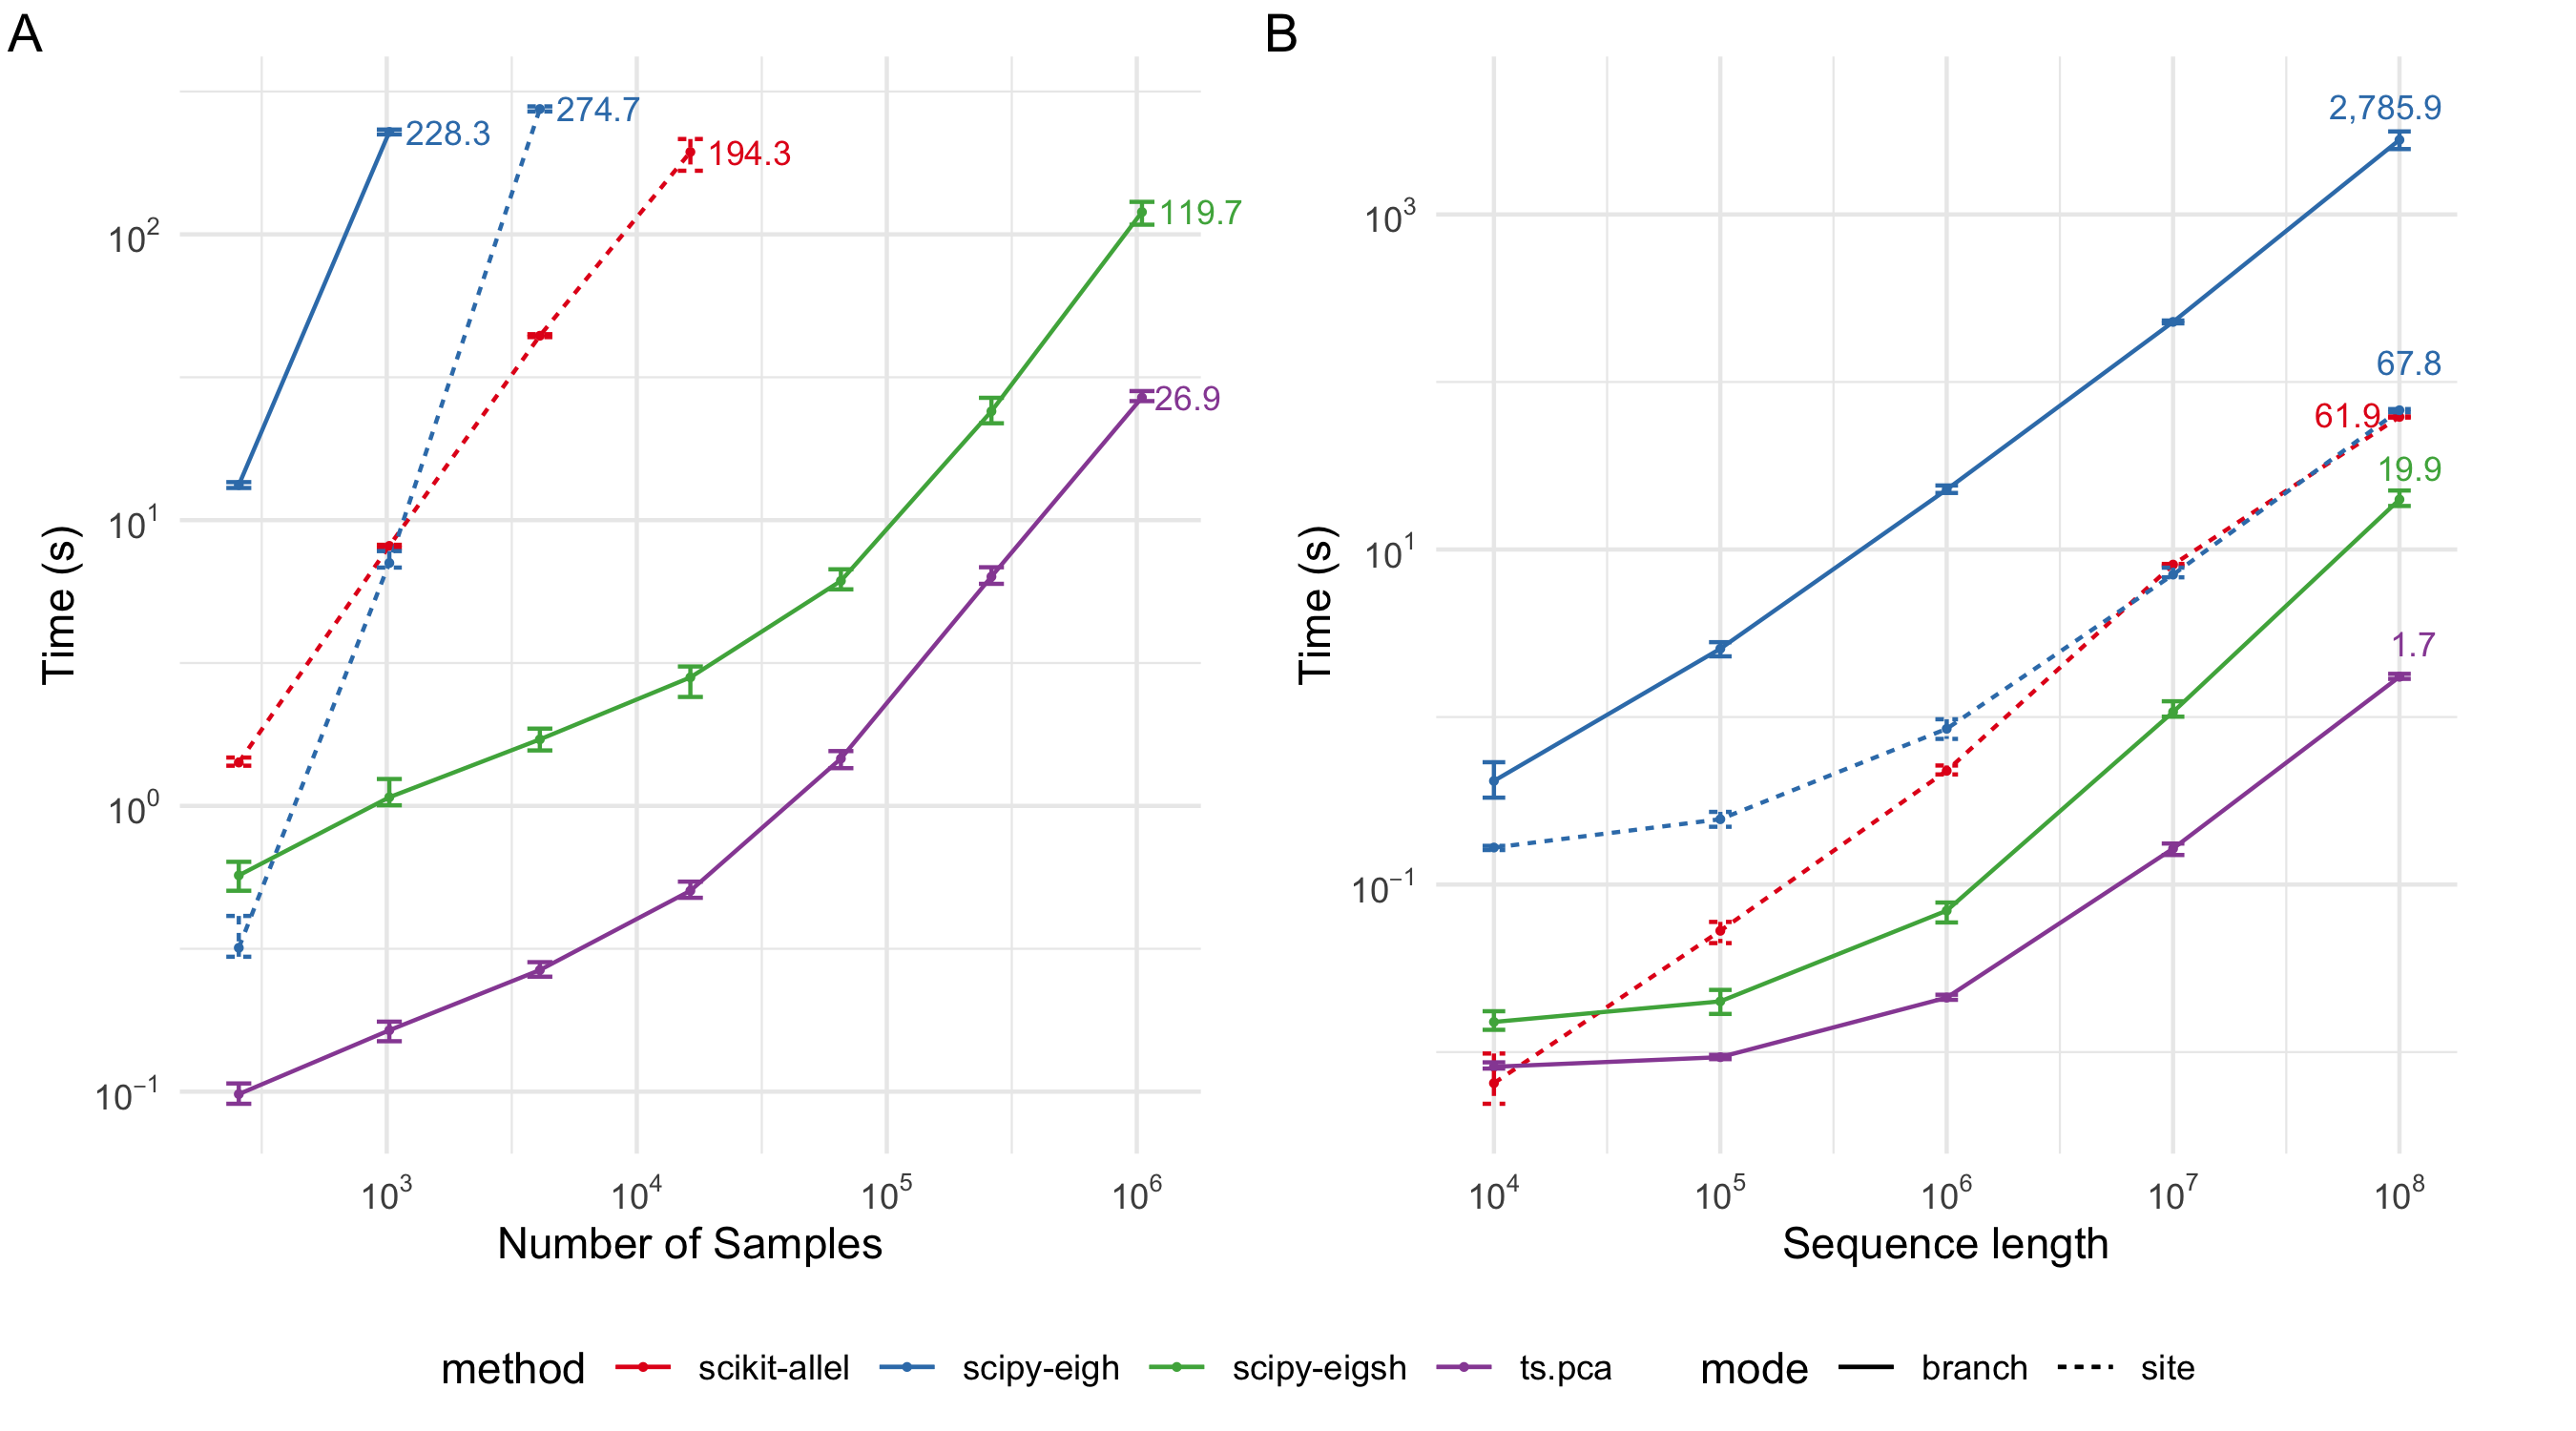
\includegraphics[width=\textwidth]{Figures/Fig2_benchmarking_plot.png}
    \label{fig:benchmarking}
    \caption{Time efficiency of different implementations of branch GRM and PCA computations.
    Each dot corresponds to the average time taken across ten simulations with different random seeds.
    Error bars represent the range in time taken across the ten simulations.
    (A) Branch GRM computation with genome sequence length fixed at $10^{7}$ and varying the number of samples.
    (B) Branch GRM computation with number of sample nodes fixed at $2^{10}$ and varying genome sequence length.
    (C) PCA with genome sequence length fixed at $10^{7}$ and varying the number of samples.
    (D) PCA with number of sample nodes fixed at $2^{10}$ and varying genome sequence length.
    Branch mode refers to branch GRM and site mode refers to genotype GRM.}
\end{figure}
\todo[inline]{Brieuc: Can you ensure the labels are shown in Fig2C for all lines (blue and red don't have them)?
Or was this "omission" intentional"? Maybe also round-off the decimal digits.}

% --- FRENCH-CANADIANS --------------------------------------------------------

\subsection{Demonstration with the French-Canadian pedigree}

To empirically illustrate the connection between pedigree and branch GRM,
we analysed the pedigree of a subset of 2,321 probands from the BALSAC dataset,
drawn from five different regions in Quebec (Figure~\ref{fig:PCA_map}G).
%
For this subset, we computed pedigree and branch GRM.
%
For the latter, we obtained an ARG from pedigree- and ancestry-informed simulation
and computed branch GRM from the ARG.
%
We simulated 100 such ARGs to evaluate the variance in branch GRM within a fixed pedigree.

\subsubsection{Principal components analyses}

% Paragraph on pedigree PCs
The overall population structure according to pedigree and branch PCA
of the 2,321 probands is shown in Figure~\ref{fig:PCA_map}
with noticeable clustering by the five regions.
%
The pedigree PCs show sharp distinctions between individuals from different regions
(Figure~\ref{fig:PCA_map}A-C).
%
Although individuals from each of the regions share a common bottleneck,
over the last four centuries,
each of the regions have drifted in their own unique way
leading to each region pulling a distinct principal component.
%
PCs 1 and 2 show a clear structure between individuals from Chaudière, Chaleur Bay, and Mistassini.
%
PCs 3 and 4 distinguish between individuals of each of the five regions except L'Assomption.
%
PCs 5 and 6 illustrate a clear distinction between L'Assomption and Chaleur Bay.
%
Only a few individuals deviated from the clusters.
\todo[inline]{Luke: are these descendants of migrants?}
\todo[inline]{Gregor: Yes. The great majority of French Canadian ancestry is attributed to French Settlers from four hundred years ago. Most settlers would have arrived in Quebec City, then radiated out from there. Each of the samples regions would have been founded by migrants who descended from these Quebec City founders.}

% Paragraph on branch PCs
The branch PCs also show the population structure (Figure~\ref{fig:PCA_map}D-F),
but there are at least two notable differences compared to pedigree PCs.
%
First, some regions clustered differently with branch PCs than with pedigree PCs.
%
This difference could be because branch PCs are based on the ARG,
which captures deeper ancestry than the pedigree,
however due to the shared bottleneck and pedigree missingness
further research is needed to study the source of these differences.
\todo[inline]{Luke: would any of these changes make sense in the light of known ancestry that is not encoded in pedigree?} 
\todo[inline]{Gregor: I'm not sure I agree with the statement "branch PCs are based on the ARG, which captures deeper ancestry than the pedigree". The ARG is based on the same information as the pedigree, if anything the pedigree has more information that the ARG because of the finite size of the genome.

If anything, I think the differences could be attributed to more noise in the ARG compared to the pedigree. The genome simulations introduce a lot of "noise" (see figure 4) and I think the PCs reflect a similar noise. 

Brieuc and I had previously identified that individuals with shallow pedigrees tend to appear at the origin of the PCA. These "shallow" individuals will be most similar to the simulated founders (EUR from the tennessen OOA model). Even though we removed individuals with very shallow genealogies, I suspect that pedigree missingness could still play a role in influencing the number of individuals near the origin of the PCA -- for both pedigree and ARG relatedness. }
%
Second, branch PCs show more variation than pedigree PCs.
%
This higher variation is partly because we have used one simulated ARG (for one chromosome)
for the branch GRM, leading to a high variance in branch PCs,
but again also because of deeper ancestry encoded in the ARG,
which pedigree does not capture.
% 
\todo[inline]{Brieuc: Confim/check/rewrite this sentence (on the one ARG used for branch GRM}
\todo[inline]{Brieuc: Could we average/sum? ~23 branch GRMs, and run PCA on that and
show that this reduces noise in branch PCs (after the initial submission!?)
Would this be another row in this plot or a plot in supplement?}
%
% When we have computed branch GRM across 23 simulated ARGs (for 23 chromosomes) within the fixed pedigree,
% the variance in corresponding branch PCs decreased (Figure~\ref{fig:PCA_map}G-I / \ref{fig:PCA_map23}).
%
\todo[inline]{Brieuc: Could we show genotype PCA compared to branch PCA in supplement?
(after the initial submission!?)}

\begin{figure}
    \centering
    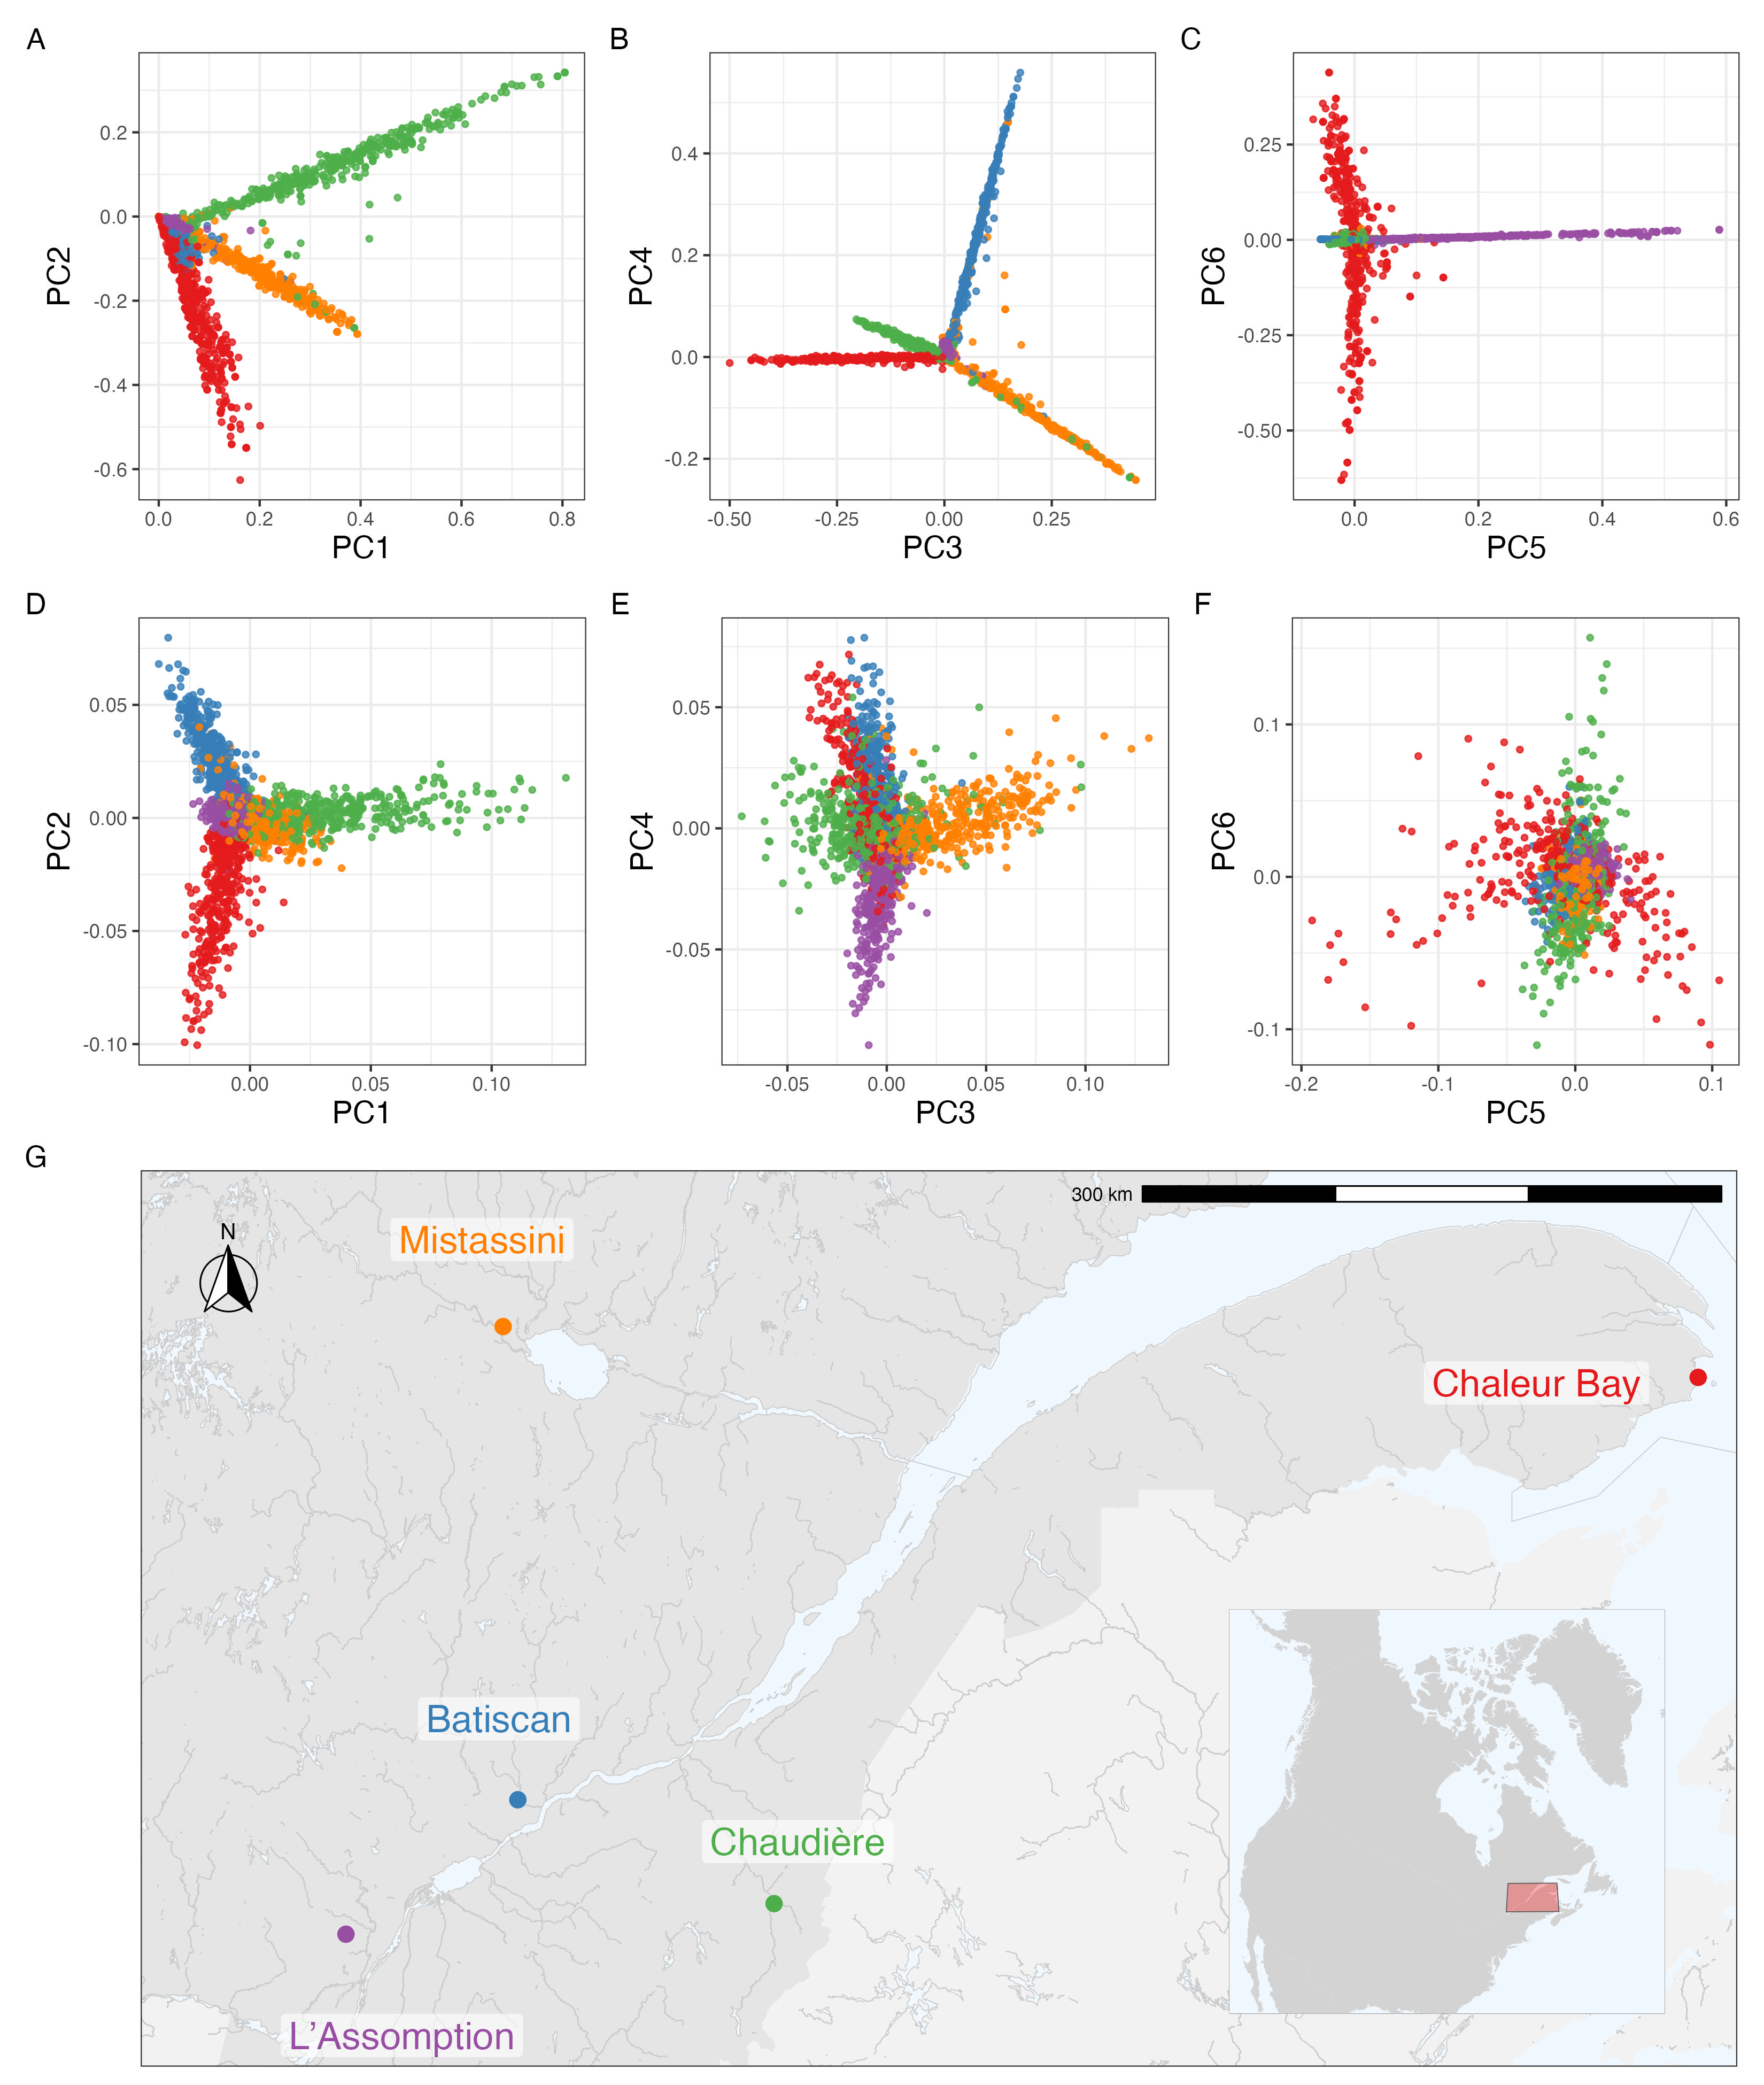
\includegraphics[width = \textwidth]{Figures/map_and_pca_grid4.jpg}
    \caption{Principal components analysis of pedigree and branch GRM of French-Canadian individuals.
    (A-C) The first six principal components of pedigree GRM.
    (D-F) The first six principal components of branch GRM.
    (G) A partial map of Quebec with approximate locations of sampled individuals. \label{fig:PCA_map}}
\end{figure}

\subsubsection{Comparing pedigree and branch GRM}

Comparison of relatedness between 250 French-Canadian individuals shows
a stronger structure with pedigree GRM than with branch GRM (Figure~\ref{fig:grm_heatmap}).
%
The difference between the two GRMs is stark
due to the randomness of genetic inheritance for a single chromosome,
which is not captured by pedigree.
%
\todo[inline]{Brieuc: Could we average/sum? ~23 branch GRMs, and show heatmap on that? (after the initial submission!?)}
% When branch GRM is computed across 23 simulated ARGs (for 23 chromosomes) within the fixed pedigree,
% the similarity between the pedigree and branch GRMs increased (Figure~\ref{fig:grm_heatmap23}).
%
Notably, when individuals have a shallow pedigree
(for example, one sampled individual from Chaleur Bay),
their corresponding pedigree GRM rows and columns have low pedigree relatedness,
while this is not the case with branch relatedness.

\begin{figure}
    \centering
    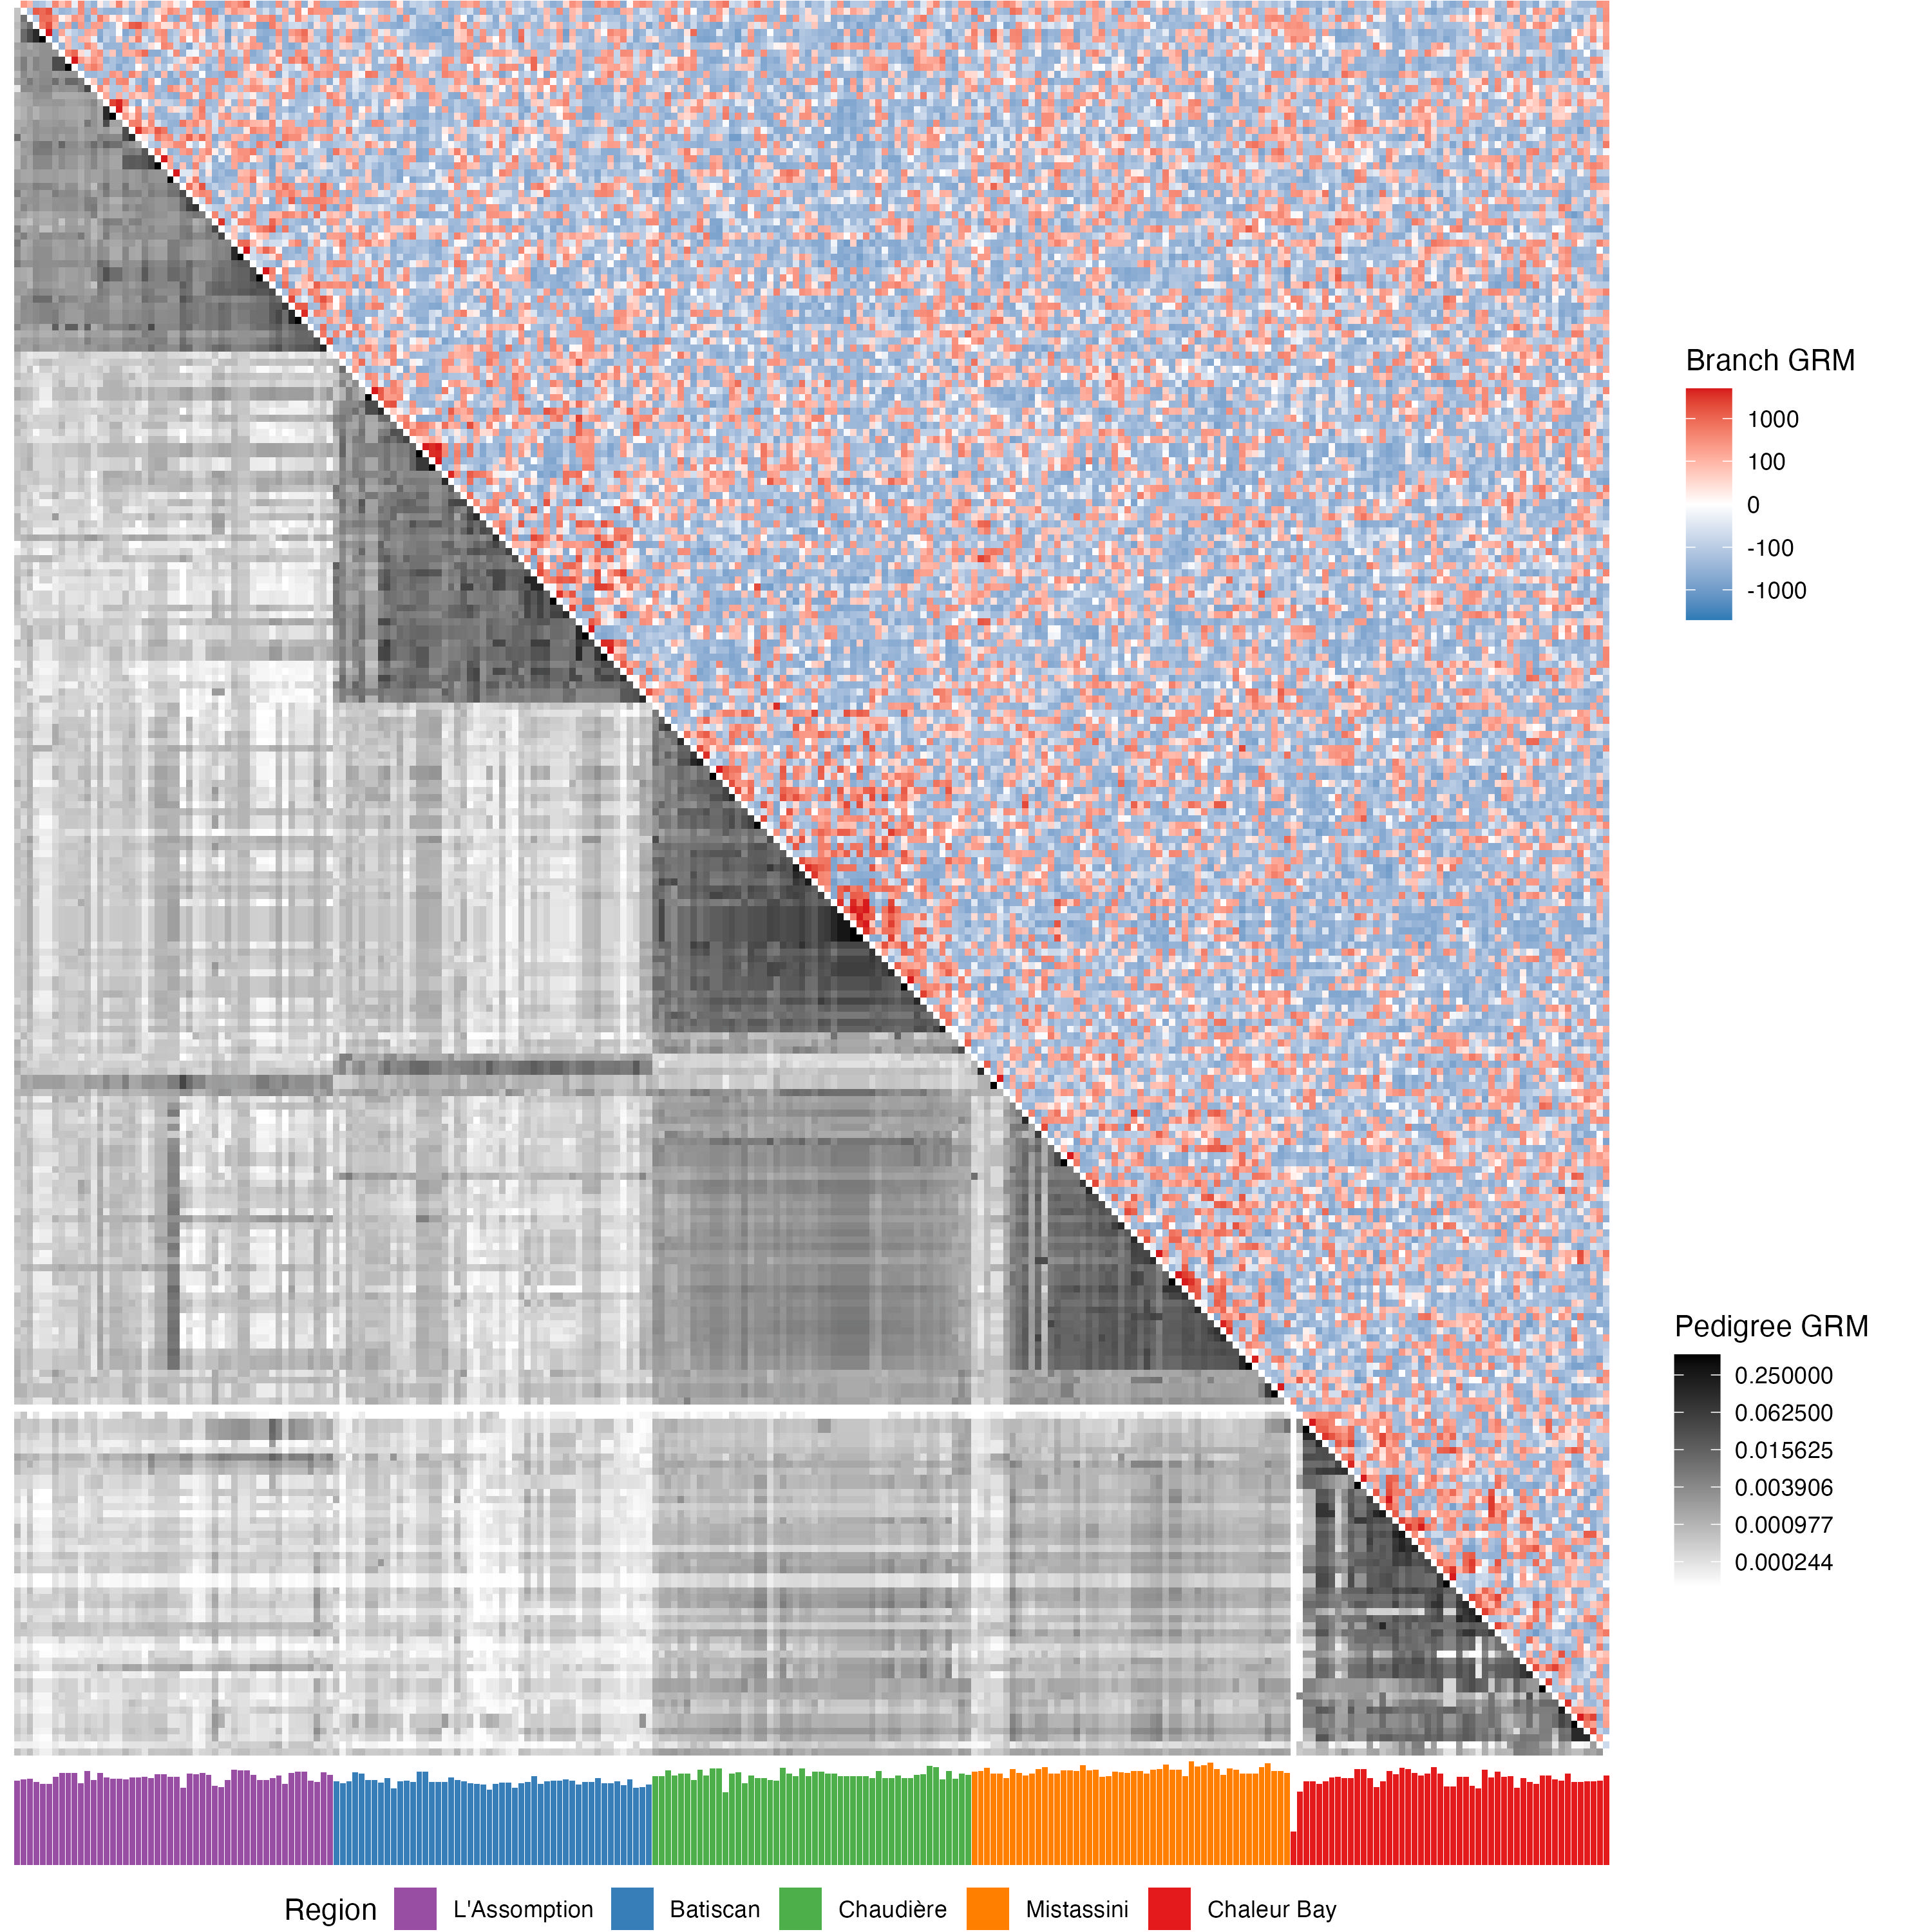
\includegraphics[width=\textwidth]{Figures/Fig4_grm_prm_heatmaps4.jpg}
    \caption{Relatedness between 250 French-Canadian individuals from 5 regions in Quebec.
      Upper-triangle: Heatmap of the branch GRM computed from one ARG (one chromosome).
      Lower-triangle: Heatmap of the pedigree GRM. 
      Bottom: Barplot of the average founder depth in the pedigree for each individual.
      The ordering of individuals is based on region and within region hierarchically on pedigree GRM.
      Because of the log scaling in the heatmap of branch GRM, we used an epsilon of 1e-4 to avoid issues with values close to zero.
    }
    \label{fig:grm_heatmap}
\end{figure}

\subsubsection{Variability in branch GRM within a fixed pedigree}

% Paragraph on main relationship between branch and pedigree relatedness
Next, we explored the variability in branch relatedness across the 100 simulated ARGs
(Figure~\ref{fig:boxplots}).
%
As expected, the branch relatedness increases with pedigree relatedness.
%
Since pedigrees are often shorter than the mean TMRCA,
and so the contribution of branch lengths within the pedigree is small,
a simple approximation of the relationship between the two
can be derived as follows.
%
First, since pedigree relatedness $r_{i,j}$ between a pair of individuals
is the expected proportion of the genome on which the two inherit from
a common ancestral genome within the pedigree,
we expect branch relatedness $C_{i,j}$ to be $r_{i,j} C_0 + (1 - r_{i,j}) C_*$,
where $C_0$ is the average branch relatedness of a genome to itself in pedigree founders,
and $C_*$ is the average branch relatedness of two distinct genomes from the pedigree founders.
%
Since this relatedness is \emph{centered}, we can (very roughly) take
$C_* \approx 0$ and $C_0 \approx A(U,U) - A(U,V)$ (with $U$ and $V$ random individuals).
%
In other words, the average centered branch relatedness
of a typical genome to itself is the total area of edges back to the roots,
minus shared edges between two typical (but different) genomes.
%
Using the relationship~\eqref{eqn:divergence_relatedness},
this is $C_0 \approx D(U,V)/2$.
%
Hence, we expect $\mathbf{B}_{i,j} \approx r_{i,j} T$
where $T$ is the mean TMRCA for two random samples from the population
(computable as one half of branch genetic divergence in \tskit{}).
%
This is shown with a line in Figure~\ref{fig:boxplots},
with $T$ computed from the demographic model used for recapitation of the pedigree.

% Paragraph on variance in branch relatedness compared to pedigree relatedness
However, there is a degree of variability in branch relatedness
between different pairs of individuals with similar pedigree relatedness.
%
While branch relatedness broadly tracks the expected relatedness outlined above,
the median relatedness varies around this value across the range of pedigree relatedness.
%
Moreover, there is substantial variability in branch relatedness within a single pair of individuals.
%
This variability is highest for sibling pairs and decreases with pedigree relatedness.

% Paragraph on summarising branch and ped relatedness
Taken together, these results illustrate that, even in a fixed pedigree,
there can be substantial variation in branch relatedness at one chromosome,
and that the degree of variation varies with respect to pedigree relatedness.
%
We emphasize that these results are obtained from simulations of a single chromosome.
%
We expect the absolute variability to decrease when considering
branch relatedness across the whole genome.

\begin{figure}
    \centering
    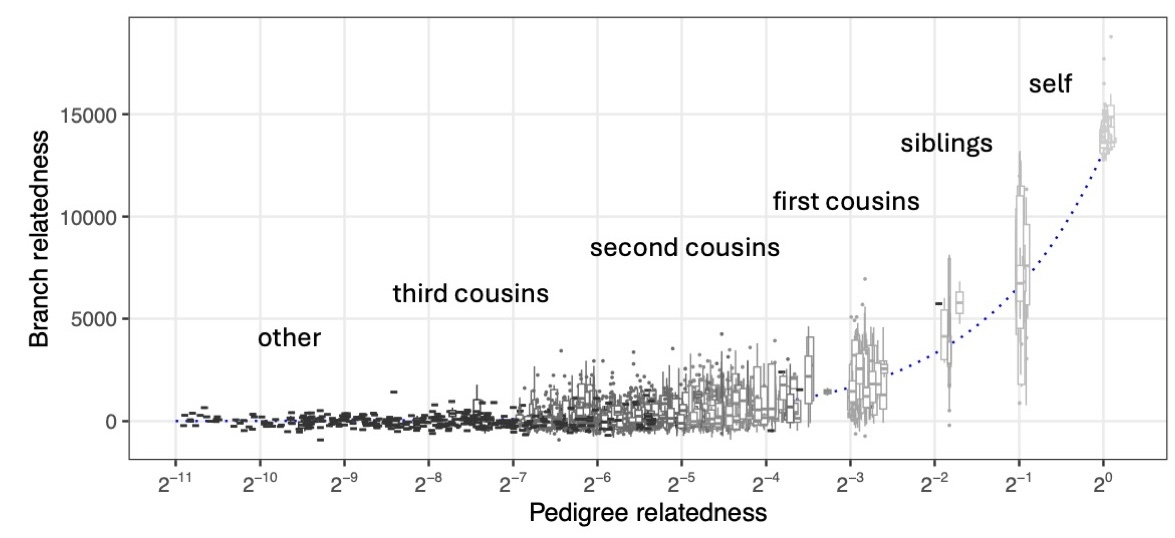
\includegraphics[width=\textwidth]{Figures/Fig5_branch_recap_sim_boxplot_combined_behind2.jpg}
    \caption{Variability in branch relatedness with respect to a fixed pedigree.
    Each box plot corresponds to a pair of individuals with pedigree relatedness
    according to some types of (pedigree) relationships (self, siblings, etc.).
    The box plot for each pair of individuals depicts variation in branch relatedness across 100 ARGs within the fixed pedigree.
    The dotted line indicates the approximate expected branch relatedness,
    which is the pedigree relatedness multiplied by the mean TMRCA among pedigree founders.}
    \label{fig:boxplots}
\end{figure}
